\def\year{2022}\relax
%File: formatting-instructions-latex-2022.tex
%release 2022.1
\documentclass[letterpaper]{article} % DO NOT CHANGE THIS
\usepackage{aaai22}  % DO NOT CHANGE THIS
\usepackage{times}  % DO NOT CHANGE THIS
\usepackage{helvet}  % DO NOT CHANGE THIS
\usepackage{courier}  % DO NOT CHANGE THIS
\usepackage[hyphens]{url}  % DO NOT CHANGE THIS
\usepackage{graphicx} % DO NOT CHANGE THIS
\urlstyle{rm} % DO NOT CHANGE THIS
\def\UrlFont{\rm}  % DO NOT CHANGE THIS
\usepackage{natbib}  % DO NOT CHANGE THIS AND DO NOT ADD ANY OPTIONS TO IT
\usepackage{caption} % DO NOT CHANGE THIS AND DO NOT ADD ANY OPTIONS TO IT
\DeclareCaptionStyle{ruled}{labelfont=normalfont,labelsep=colon,strut=off} % DO NOT CHANGE THIS
\frenchspacing  % DO NOT CHANGE THIS
\setlength{\pdfpagewidth}{8.5in}  % DO NOT CHANGE THIS
\setlength{\pdfpageheight}{11in}  % DO NOT CHANGE THIS
%


\usepackage{algorithm}
\usepackage{algorithmic}

\usepackage{amsmath} 
\usepackage{amssymb}
\usepackage{amsthm}

\usepackage{xcolor}
\usepackage{subcaption}
\usepackage{breqn}
\usepackage{subfiles}
\usepackage{microtype}
\usepackage{multirow}
\usepackage{booktabs}
\usepackage{bbm}
\usepackage[group-separator={,}]{siunitx}

\setcounter{table}{0}
\renewcommand{\thetable}{R\arabic{table}}

\setcounter{figure}{0}
\renewcommand{\thefigure}{R\arabic{figure}}

% These are recommended to typeset algorithms but not required. See the subsubsection on algorithms. Remove them if you don't have algorithms in your paper.
\usepackage{algorithm}
\usepackage{algorithmic}
\newcommand{\sysname}{\textsc{NestedMAML}}
%
% These are are recommended to typeset listings but not required. See the subsubsection on listing. Remove this block if you don't have listings in your paper.
\usepackage{newfloat}
\usepackage{listings}
\lstset{%
	basicstyle={\footnotesize\ttfamily},% footnotesize acceptable for monospace
	numbers=left,numberstyle=\footnotesize,xleftmargin=2em,% show line numbers, remove this entire line if you don't want the numbers.
	aboveskip=0pt,belowskip=0pt,%
	showstringspaces=false,tabsize=2,breaklines=true}
\floatstyle{ruled}
\newfloat{listing}{tb}{lst}{}
\floatname{listing}{Listing}
%
%\nocopyright
%
% PDF Info Is REQUIRED.
% For /Title, write your title in Mixed Case.
% Don't use accents or commands. Retain the parentheses.
% For /Author, add all authors within the parentheses,
% separated by commas. No accents, special characters
% or commands are allowed.
% Keep the /TemplateVersion tag as is
\pdfinfo{
/Title (AAAI Press Formatting Instructions for Authors Using LaTeX -- A Guide)
/Author (AAAI Press Staff, Pater Patel Schneider, Sunil Issar, J. Scott Penberthy, George Ferguson, Hans Guesgen, Francisco Cruz, Marc Pujol-Gonzalez)
/TemplateVersion (2022.1)
}

% DISALLOWED PACKAGES
% \usepackage{authblk} -- This package is specifically forbidden
% \usepackage{balance} -- This package is specifically forbidden
% \usepackage{color (if used in text)
% \usepackage{CJK} -- This package is specifically forbidden
% \usepackage{float} -- This package is specifically forbidden
% \usepackage{flushend} -- This package is specifically forbidden
% \usepackage{fontenc} -- This package is specifically forbidden
% \usepackage{fullpage} -- This package is specifically forbidden
% \usepackage{geometry} -- This package is specifically forbidden
% \usepackage{grffile} -- This package is specifically forbidden
% \usepackage{hyperref} -- This package is specifically forbidden
% \usepackage{navigator} -- This package is specifically forbidden
% (or any other package that embeds links such as navigator or hyperref)
% \indentfirst} -- This package is specifically forbidden
% \layout} -- This package is specifically forbidden
% \multicol} -- This package is specifically forbidden
% \nameref} -- This package is specifically forbidden
% \usepackage{savetrees} -- This package is specifically forbidden
% \usepackage{setspace} -- This package is specifically forbidden
% \usepackage{stfloats} -- This package is specifically forbidden
% \usepackage{tabu} -- This package is specifically forbidden
% \usepackage{titlesec} -- This package is specifically forbidden
% \usepackage{tocbibind} -- This package is specifically forbidden
% \usepackage{ulem} -- This package is specifically forbidden
% \usepackage{wrapfig} -- This package is specifically forbidden
% DISALLOWED COMMANDS
% \nocopyright -- Your paper will not be published if you use this command
% \addtolength -- This command may not be used
% \balance -- This command may not be used
% \baselinestretch -- Your paper will not be published if you use this command
% \clearpage -- No page breaks of any kind may be used for the final version of your paper
% \columnsep -- This command may not be used
% \newpage -- No page breaks of any kind may be used for the final version of your paper
% \pagebreak -- No page breaks of any kind may be used for the final version of your paperr
% \pagestyle -- This command may not be used
% \tiny -- This is not an acceptable font size.
% \vspace{- -- No negative value may be used in proximity of a caption, figure, table, section, subsection, subsubsection, or reference
% \vskip{- -- No negative value may be used to alter spacing above or below a caption, figure, table, section, subsection, subsubsection, or reference

\setcounter{secnumdepth}{0} %May be changed to 1 or 2 if section numbers are desired.

% The file aaai22.sty is the style file for AAAI Press
% proceedings, working notes, and technical reports.
%

% Title

% Your title must be in mixed case, not sentence case.
% That means all verbs (including short verbs like be, is, using,and go),
% nouns, adverbs, adjectives should be capitalized, including both words in hyphenated terms, while
% articles, conjunctions, and prepositions are lower case unless they
% directly follow a colon or long dash
\title{AAAI Press Formatting Instructions \\for Authors Using \LaTeX{} --- A Guide}
\author{
    %Authors
    % All authors must be in the same font size and format.
    Written by AAAI Press Staff\textsuperscript{\rm 1}\thanks{With help from the AAAI Publications Committee.}\\
    AAAI Style Contributions by Pater Patel Schneider,
    Sunil Issar,\\
    J. Scott Penberthy,
    George Ferguson,
    Hans Guesgen,
    Francisco Cruz\equalcontrib,
    Marc Pujol-Gonzalez\equalcontrib
}
\affiliations{
    %Afiliations
    \textsuperscript{\rm 1}Association for the Advancement of Artificial Intelligence\\
    % If you have multiple authors and multiple affiliations
    % use superscripts in text and roman font to identify them.
    % For example,

    % Sunil Issar, \textsuperscript{\rm 2}
    % J. Scott Penberthy, \textsuperscript{\rm 3}
    % George Ferguson,\textsuperscript{\rm 4}
    % Hans Guesgen, \textsuperscript{\rm 5}.
    % Note that the comma should be placed BEFORE the superscript for optimum readability

    2275 East Bayshore Road, Suite 160\\
    Palo Alto, California 94303\\
    % email address must be in roman text type, not monospace or sans serif
    publications22@aaai.org
%
% See more examples next
}

%Example, Single Author, ->> remove \iffalse,\fi and place them surrounding AAAI title to use it
\iffalse
\title{My Publication Title --- Single Author}
\author {
    Author Name
}
\affiliations{
    Affiliation\\
    Affiliation Line 2\\
    name@example.com
}
\fi

\iffalse
%Example, Multiple Authors, ->> remove \iffalse,\fi and place them surrounding AAAI title to use it
\title{My Publication Title --- Multiple Authors}
\author {
    % Authors
    First Author Name,\textsuperscript{\rm 1}
    Second Author Name, \textsuperscript{\rm 2}
    Third Author Name \textsuperscript{\rm 1}
}
\affiliations {
    % Affiliations
    \textsuperscript{\rm 1} Affiliation 1\\
    \textsuperscript{\rm 2} Affiliation 2\\
    firstAuthor@affiliation1.com, secondAuthor@affilation2.com, thirdAuthor@affiliation1.com
}
\fi


% REMOVE THIS: bibentry
% This is only needed to show inline citations in the guidelines document. You should not need it and can safely delete it.
\usepackage{bibentry}
% END REMOVE bibentry

\begin{document}
\section{General response}
% \vspace{-1ex}
Thank you all reviewers for the valuable comments. For Reproducibility, we actually have an anonymous link to the code in page 6, and the supplementary material attached in the same pdf document shows all necessary proofs.

{\color{blue} {\noindent}Q1: weight distribution? }
We show the weight distribution and weight trends for different OOD ratios (SVHN 30\%, 60\%, 90\%) in Figure~\ref{fig:additional_weights_dist}. Compared to 90\% OOD, the weights under 30\% and 60\% would become more stable earlier. {\color{blue}{\noindent}Q2: 5-way 1-shot experiments? } We show 1-shot experiments for two OOD datasets for 30\%, 60\% in Table~\ref{tab:additonal_5w1s} (using the same hyperparameters). The results show that \sysname{} still outperforms MAML by around 2\%. {\color{blue}{\noindent}Q3: Experiments on more datasets? }We show additional results on CUB-200-2011 and tieredImageNet datasets with FashionMNIST as OOD dataset and 90\% OOD ratio in Table~\ref{tab:additonal}. From the results, it is evident that \sysname{} achieves better performance compared to MAML (at least 5\% improvement).

\begin{table}[t!]
% \footnotesize
% \vspace{-3mm}
    \tiny  
    % \vspace{-3mm}
    \centering
    \begin{center}
    \vspace{-3mm}
    \begin{tabular}{l | c c |c c }
        \toprule
         & \multicolumn{2}{c|}{\textbf{CUB-200}} & \multicolumn{2}{c}{\textbf{tieredImageNet}}\\
        % \Xhline{2\arrayrulewidth}
        % &\multicolumn{3}{c}{\textbf{5-way 3-shot}} \\
        Dataset  & 3-shot & 5-shot  & 3-shot & 5-shot  \\
        \midrule
        MAML-OOD-RM (Skyline) & 61.75\% & 69.67\% & 58.71\%  & 65.62\% \\
        \midrule
        MAML              & 53.23\% & 61.84\% & 49.74\%  & 56.45\%  \\
        \hline
        \sysname{} (ours) & \textbf{59.18}\% & \textbf{68.53}\% & \textbf{57.17}\%  & \textbf{64.91}\% \\
        \bottomrule 
        % \Xhline{2\arrayrulewidth}
    \end{tabular}
\vspace{-3mm}
\end{center}
\vspace{-1mm}
\caption{\small 90\% FashionMNIST OOD.}
\label{tab:additonal}
\end{table}

\begin{table}[t!]
% \footnotesize
% \vspace{-3mm}
    \tiny  
    % \vspace{-3mm}
    \centering
    \begin{center}
    \vspace{-3mm}
    \begin{tabular}{l | c c |c c }
        \toprule
         & \multicolumn{2}{c|}{\textbf{SVHN}} & \multicolumn{2}{c}{\textbf{FashionMNIST}}\\
        % \Xhline{2\arrayrulewidth}
        % &\multicolumn{3}{c}{\textbf{5-way 3-shot}} \\
        OOD Dataset  & 30\% & 60\%  & 30\% & 60\%  \\
        \midrule
        MAML-OOD-RM (Skyline)       & 46.62\% & 45.70\% & 46.62\%  & 45.70\% \\
        \midrule
        MAML              & 41.07\% & 38.16\% & 39.73\%  & 38.65\%  \\
        \hline
        \sysname{} (ours) & \textbf{43.18}\% & \textbf{41.30}\% & \textbf{42.43}\%  & \textbf{40.81}\% \\
        \bottomrule 
        % \Xhline{2\arrayrulewidth}
    \end{tabular}
\vspace{-3mm}
\end{center}
\vspace{-1mm}
\caption{\small 5-way 1-shot experiments for two OOD datasets.}
\label{tab:additonal_5w1s}
\end{table}


\begin{figure}[!t]
\vspace{-3mm}
%\captionsetup[subfigure]{aboveskip=-1pt,belowskip=-2pt}
    \centering
    \begin{subfigure}[b]{0.23\textwidth}
        \centering
        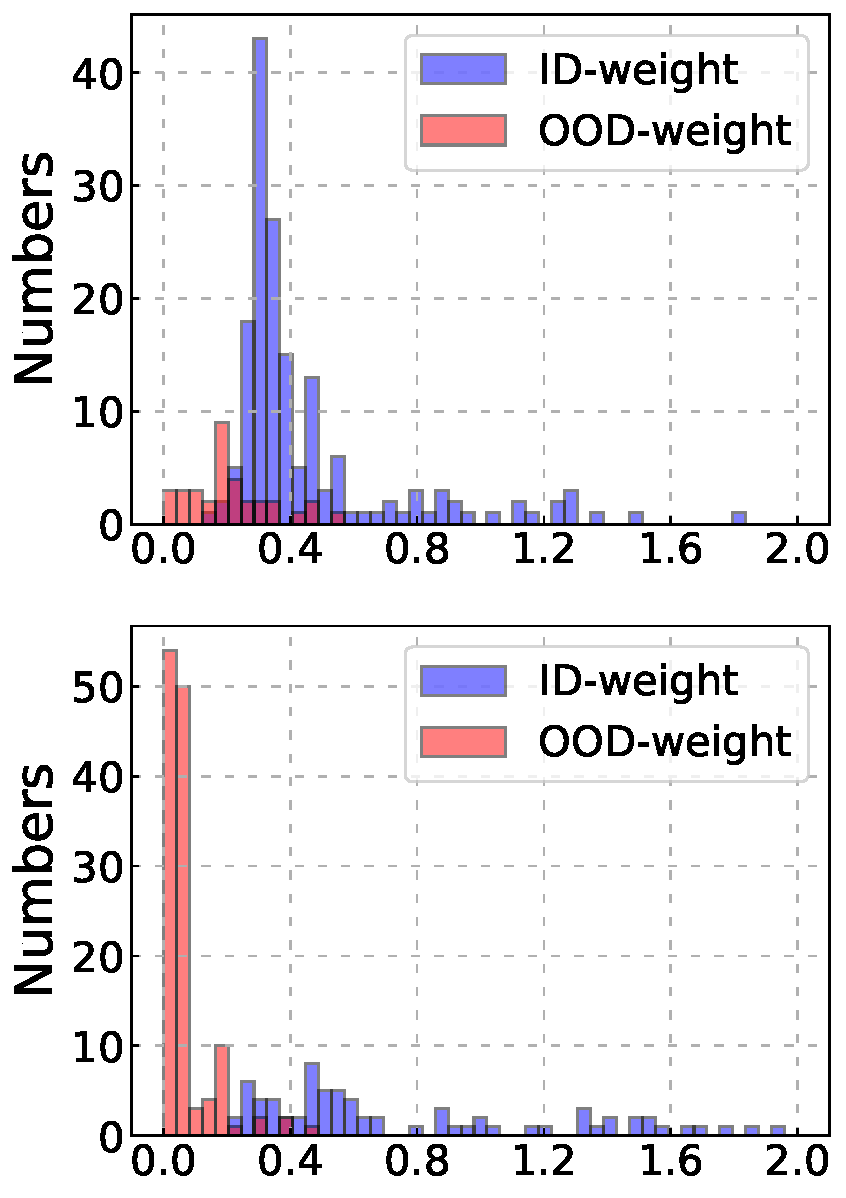
\includegraphics[width=\linewidth, height=5cm]{Robust Meta Learning/figs/svhn-5-oodthreeOOD-crop.pdf}
        \caption{Numbers vs. Weights}
    \end{subfigure}
    \begin{subfigure}[b]{0.23\textwidth}
        \centering
        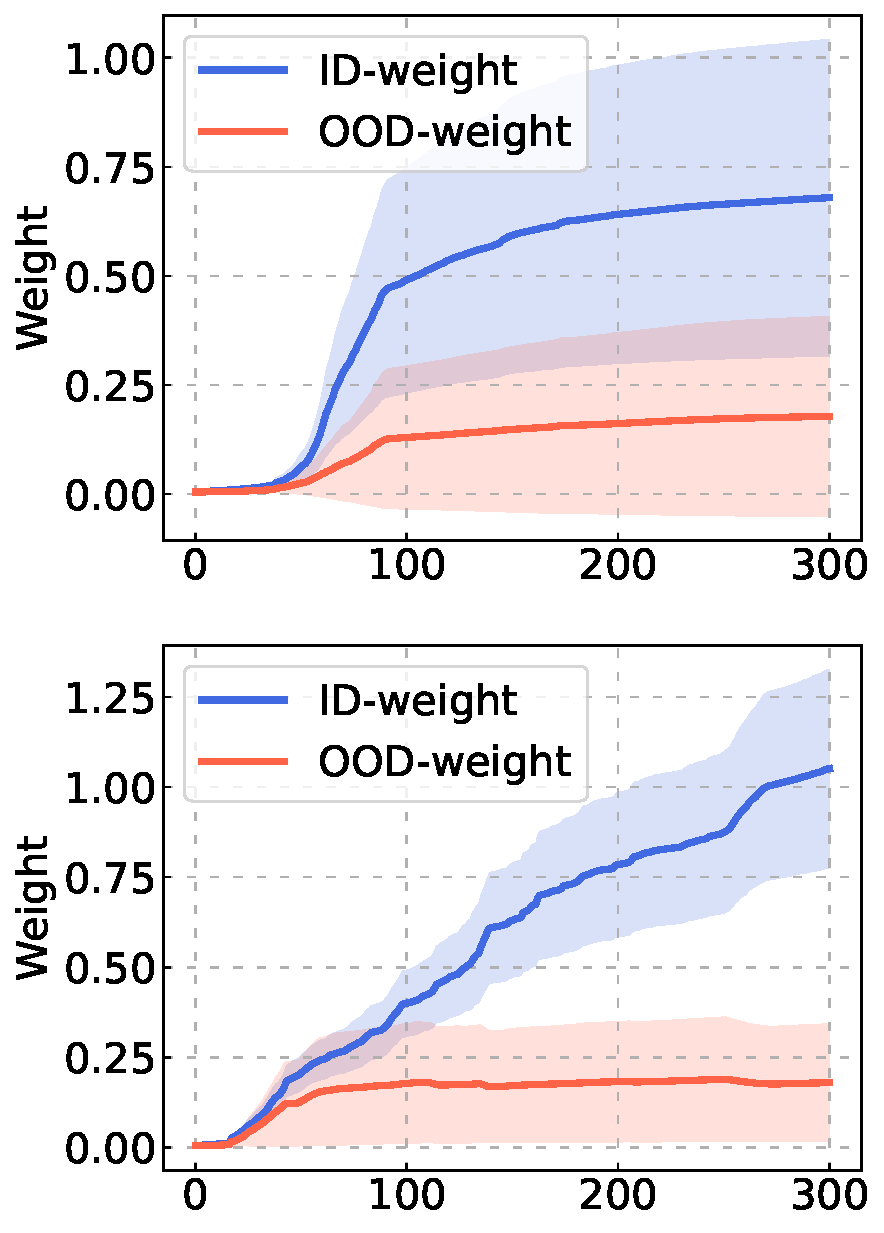
\includegraphics[width=\linewidth, height=5cm]{Robust Meta Learning/figs/Comb_curve_svhn-5-oodthreeOOD_crop.pdf}
        \caption{Weights vs. Iterations$*$100}
    \end{subfigure}
    \vspace{-3mm}
    \caption{\small (a) Task weight distribution under 30\% (top), 60\% (bottom) OOD ratio (SVHN, 5-shot). 90\% OOD ratio case is shown in Figure 3 of the main paper. (b) Weights changing with iteration under 60\% (top), 90\% (bottom) OOD ratio (SVHN, 5-shot). 30\% OOD ratio case is shown in Figure 4 of the main paper.}
    \label{fig:additional_weights_dist}
\vspace{-2mm}
\end{figure}
\vspace{-3mm}

\section{Response to Reviewer 1}
% \vspace{-1ex}
{\color{blue}Q1: \sysname{} vs. MAML in general few-shot learning?} The proposed method works similarly to MAML in the general few-shot learning scenario. Still, the key advantage of our proposed method is that it achieves faster convergence to optimal accuracy compared to MAML. {\noindent}{\color{blue}Q2: Weight distributions?} Please refer to Q1 in General response. {\noindent}{\color{blue}Q3: Experiments on Omniglot or tiered-ImageNet.} Please refer to Q3 in General response.
\vspace{-3mm}
\section{Response to Reviewer 2}
% \vspace{-1ex}
{\color{blue}Q1: Notation $\phi$?}
$\phi$ is the adapted model parameters for the specific task. It is optimized through one-step gradient descent, which is basically Eq.(1): $\phi = \mathcal{A}lg(\boldsymbol{\theta}, \mathcal{D}_{i}^{S}) = \boldsymbol{\theta} - \alpha \nabla_{\boldsymbol{\theta}}\mathcal{L}(\boldsymbol{\theta}, \mathcal{D}_{i}^{S})$. We mentioned this in Lemma 1 in page 4. {\color{blue}{\noindent}Q2: How will $\alpha$ be involved in Eq. (5)?}
$\alpha$ is involved in Eq.(2), which Eq.(5) used. As you kindly suggested, we will mention Eq.(2) and add it to the Algorithm in the new version. {\noindent}{\color{blue}Q3: Weights distribution?}
Please see Q1 in General response. {\noindent}{\color{blue}Q4: Literature for hyperparameter optimization methods?} We will add details on the relationship with hyperparameter optimization methods to the related work in the new version. {\noindent}{\color{blue}Q5: Task clustering method?} In our experiments, we use task clustering for Table 1 and Table 2 experiments where we cluster tasks into 200 clusters and share the same weight among all tasks in the cluster. As for experiments in Table 3, we use instance-level weighting with an individual weight for each sample and has no weight sharing. We agree that the description of task clustering is not concise and will add a detailed description of task clustering and its usage in the next version.{\noindent} {\color{blue} Q6: Challenging datasets for experiments?} Please refer to Q3 in General response.
\vspace{-3mm}
\section{Response to Reviewer 4}
% \vspace{-1ex}

{\noindent {\color{blue}Q1: Novelty?}} To our knowledge, our work is the first to propose a nested bilevel optimization method and provide a functional approach. Furthermore, our work contributed theoretically by proving the convergence rate of methods trained using the nested bi-level optimization method for convex loss functions. {\noindent}{\color{blue}Q2: 1-shot experiments? }Please refer to Q2 in General response. {\noindent}{\color{blue}Q3: Computational time comparison? } We only presented the comparison between our method and MAML on comptuational time in our paper, as other baselines are slower than MAML. We will add a detailed comparison of the computation time of all baselines used with \sysname{} in the next version of the paper.{\noindent} {\color{blue}Q4: Evidence for model-agnosticness? }Similar to MAML(Model-agnostic Meta-Learning), \sysname{} is compatible with any model that can be trained with gradient descent. Hence, we call it model agnostic.
\vspace{-3mm}
\section{Response to Reviewer 5}
% \vspace{-1ex}
{\color{blue}Q1: More adaption steps in reweighting?} \sysname{} performs better with more adaptation steps, but the increase in steps increases the computational cost, resulting in a performance-efficiency tradeoff. Our experiments, however, indicate that the performance improvement does not justify the associated increase in computation cost, so we consider the one-step update in our work. {\noindent}{\color{blue}Q2: 1-shot experiments? } Please refer to Q2 in General response. {\noindent}{\color{blue}Q3: Convergence for non-convex loss functions? }We will work on the convergence rate of \sysname{} for non-convex loss functions in the next version of the paper. {\noindent}{\color{blue}Q4: More OOD generalization baselines? } In our work, we predominantly concentrated on MAML based variants for OOD generalization. We will add non-MAML OOD generalization methods as baselines in the next version of the paper.


% Use \bibliography{yourbibfile} instead or the References section will not appear in your paper
\nobibliography{aaai22}
\end{document}
